\documentclass{resume}
\usepackage{graphicx}
\usepackage{tabu}
\usepackage{multirow}
\usepackage{progressbar}

\usepackage{zh_CN-Adobefonts_external} % Simplified Chinese Support using external fonts (./fonts/zh_CN-Adobe/)
\usepackage{linespacing_fix} % disable extra space before next section
\usepackage{cite}
\usepackage{graphicx} % 确保你已经加载了 graphicx 包（用于插入图片）
\begin{document}
\pagenumbering{gobble} % suppress displaying page number

\name{邹杰}

\normalsize
\begin{tabu}{ l c r }  % 左对齐、居中、右对齐
  \textbf{ } & & 
 \multirow{3}{1in}{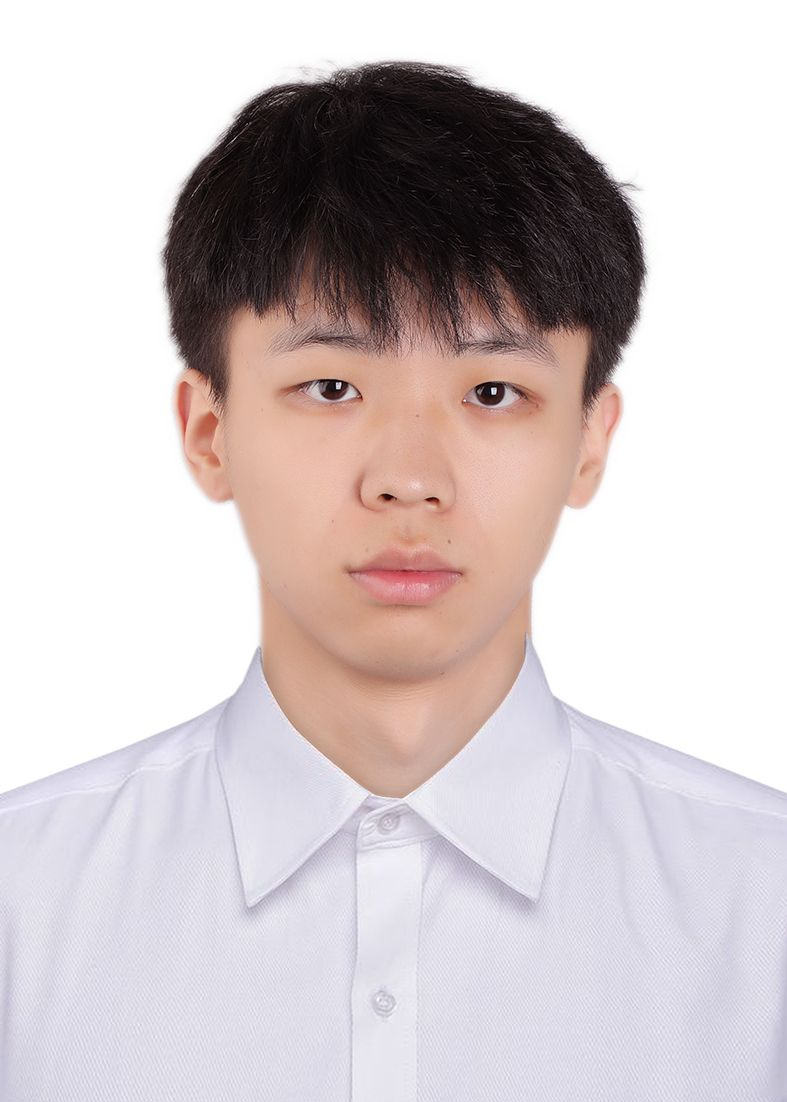
\includegraphics[width=0.57in]{picture}} \\
  
  \email{1991645643@qq.com} \textperiodcentered\ 
  \phone{(+86) 18684144634} & & \\
  
  \textbf{期望岗位：} 软件开发工程师 \textperiodcentered\ 
  \textbf{期望城市：} 上海\textperiodcentered\phantom{11111111111111111111111111111111}& & \\
\end{tabu}

 
\section{\faGraduationCap\  教育背景}
\datedsubsection{\textbf{华中科技大学}, 武汉}{2023 -- 至今}
\small\textit{在读硕士研究生}\ 计算机科学与技术学院, 计算机技术 
\datedsubsection{\textbf{南京邮电大学}, 南京}{2019 -- 2023}
\small\textit{学士}\ 软件学院，软件工程

\section{\faCogs\ 专业技能}
% increase linespacing [parsep=0.5ex]
\begin{itemize}[parsep=0.5ex]
  \item 熟练掌握 C/C++，熟悉面向对象编程思想，熟练使用 STL 常用容器和 C++11 特性
  \item 熟悉 Linux 系统编程，包括多线程、IO 多路复用、epoll 等技术
  \item 熟悉常用数据结构与算法，掌握操作系统、计算机网络等基础知识
  \item 熟练使用 MySQL，了解索引、事务、锁机制及存储引擎原理
  \item 熟悉 Git、VSCode 等开发工具
\end{itemize}

\section{\faUsers\ 项目经历}

\datedsubsection{\textbf{C++服务器框架－协程库}}{2025年4月 -- 2025年6月}
\role{个人项目，C++，多线程，协程}

\begin{itemize}
  \item 项目内容：独立开发基于 Linux 的 C++ 服务器框架，核心实现协程调度模块
  \item 项目实施：
    \begin{enumerate}[label=\arabic*. ]
      \item 封装线程：基于 RAII 思想，实现互斥锁、信号量、读写锁等线程同步机制
      \item 实现协程：使用 ucontext_t 实现非对称协程，定义三种协程状态，实现子协程与主线程的切换
      \item 实现定时器：基于时间堆实现定时器功能，支持定时事件管理
      \item 实现协程调度器：设计 N-M 协程调度器，主线程参与调度，结合 epoll 和定时器实现 I/O 协程调度
      \item Hook 封装：对 sleep、Socket IO、fd 操作等系统调用进行 Hook，将阻塞调用转换为异步操作
    \end{enumerate}
  \item 项目测试：分别使用原生 epoll、libevent 与本项目实现简易服务器，单线程性能相近，多线程、IO 密集场景下表现更优
\end{itemize}

\datedsubsection{\textbf{基于Linux平台的轻量级应用服务器} }{2025年1月 -- 2025年4月}
\role{个人项目}{c++，http服务器，Linux}

\begin{itemize}
  \item 项目内容：设计并实现一个基于 Linux 平台的轻量级 HTTP 服务器
  \item 项目实施：
    \begin{enumerate}[label=\arabic*. ]
      \item 高效事件处理：使用 epoll 实现事件监听与处理，提升服务器并发能力
      \item 高并发模型：采用 Reactor 模型，实现 One Loop per Thread，支持多客户端并发连接
      \item 动态缓冲区：实现自动增长缓冲区，动态调整大小以适配不同请求，优化内存分配
      \item 连接管理：使用小根堆实现高效定时器，管理连接超时时间，防止空闲连接资源浪费
      \item 异步日志：设计异步日志模块，基于单例模式和阻塞队列实现高效日志写入
    \end{enumerate}
   \item 项目测试：使用 webbench 发起 1000 个并发进程，对服务器进行 60 秒压力测试，短连接 QPS 为 1.8 万，长连接 QPS 达 5.2 万
\end{itemize}

\section{\faInfo\ 个人评价}
% increase linespacing [parsep=0.5ex]
\begin{itemize}[parsep=0.5ex]
  \item 学习能力强，能快速掌握新知识和技能
  \item 工作认真负责，具备良好的团队协作意识
  \item 性格乐观开朗，具备较强的抗压能力和沟通能力
\end{itemize}

\end{document}